\documentclass{standalone}
\usepackage{tikz}
\usetikzlibrary{patterns, positioning}

\begin{document}
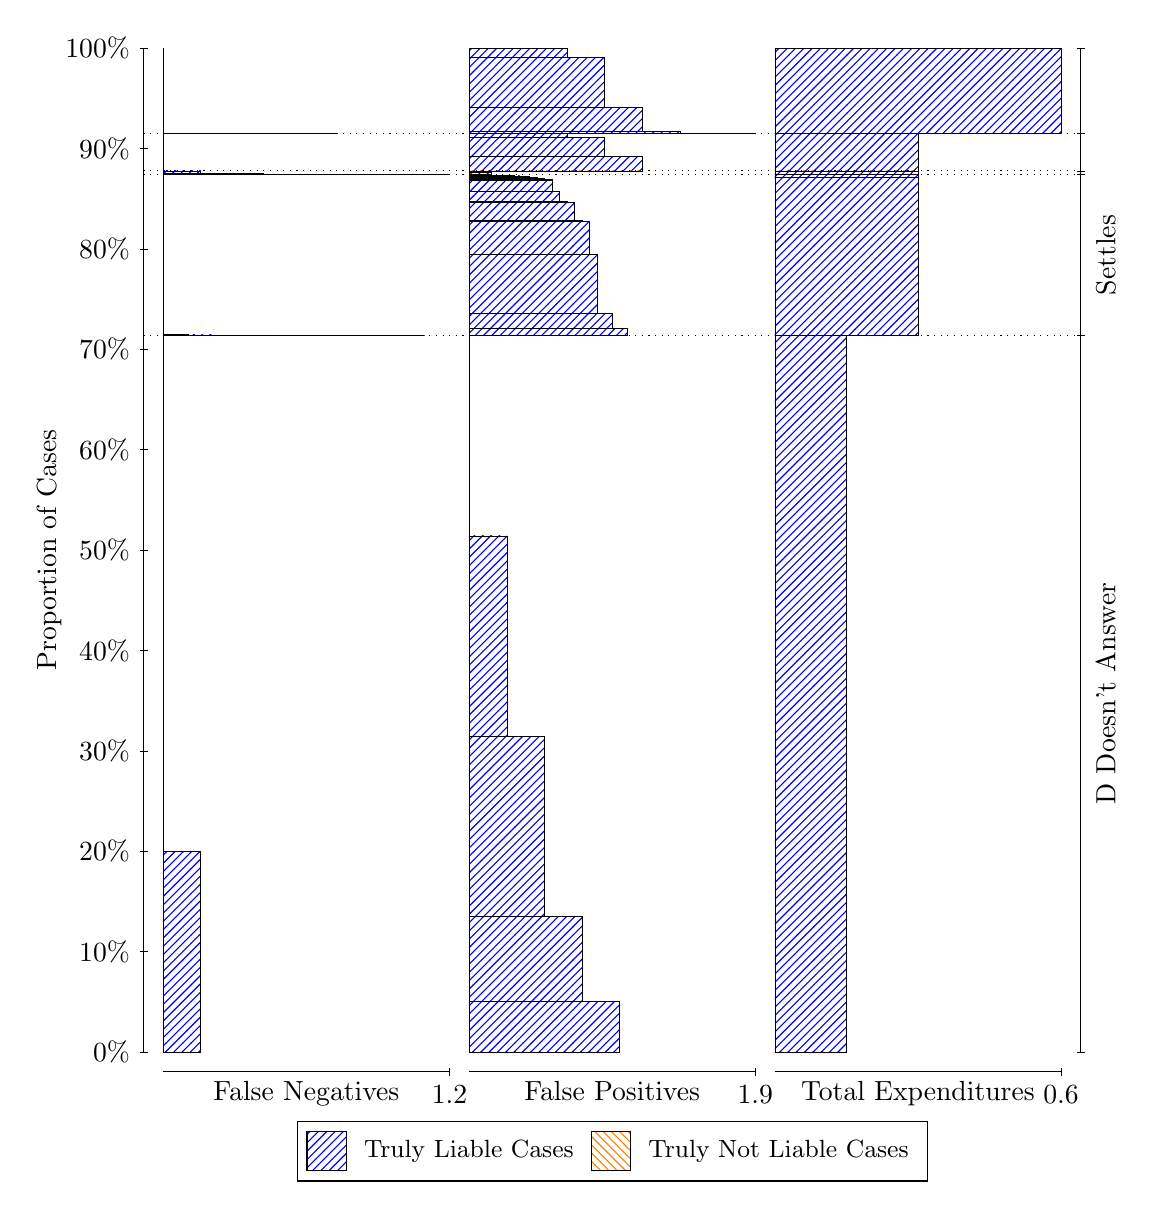
\begin{tikzpicture}
\draw[black, very thin] (1.5,1.75) -- (1.5,14.5);
\node[rotate=90, anchor=center] at (0.3, 8.125) {Proportion of Cases};
\draw[black, very thin] (1.45,1.75) -- (1.55,1.75);
\node[anchor=east] at (1.45, 1.75) {0\%};
\draw[black, very thin] (1.45,3.025) -- (1.55,3.025);
\node[anchor=east] at (1.45, 3.025) {10\%};
\draw[black, very thin] (1.45,4.3) -- (1.55,4.3);
\node[anchor=east] at (1.45, 4.3) {20\%};
\draw[black, very thin] (1.45,5.575) -- (1.55,5.575);
\node[anchor=east] at (1.45, 5.575) {30\%};
\draw[black, very thin] (1.45,6.85) -- (1.55,6.85);
\node[anchor=east] at (1.45, 6.85) {40\%};
\draw[black, very thin] (1.45,8.125) -- (1.55,8.125);
\node[anchor=east] at (1.45, 8.125) {50\%};
\draw[black, very thin] (1.45,9.4) -- (1.55,9.4);
\node[anchor=east] at (1.45, 9.4) {60\%};
\draw[black, very thin] (1.45,10.675) -- (1.55,10.675);
\node[anchor=east] at (1.45, 10.675) {70\%};
\draw[black, very thin] (1.45,11.95) -- (1.55,11.95);
\node[anchor=east] at (1.45, 11.95) {80\%};
\draw[black, very thin] (1.45,13.225) -- (1.55,13.225);
\node[anchor=east] at (1.45, 13.225) {90\%};
\draw[black, very thin] (1.45,14.5) -- (1.55,14.5);
\node[anchor=east] at (1.45, 14.5) {100\%};

\draw[black, very thin] (13.4,1.75) -- (13.4,14.5);
\draw[black, very thin] (13.35,1.75) -- (13.45,1.75);
\node[anchor=west] at (13.35, 1.75) {};
\draw[black, very thin] (13.35,10.853) -- (13.45,10.853);
\node[anchor=west] at (13.35, 10.853) {};
\draw[black, very thin] (13.35,12.891) -- (13.45,12.891);
\node[anchor=west] at (13.35, 12.891) {};
\draw[black, very thin] (13.35,12.941) -- (13.45,12.941);
\node[anchor=west] at (13.35, 12.941) {};
\draw[black, very thin] (13.35,13.415) -- (13.45,13.415);
\node[anchor=west] at (13.35, 13.415) {};
\draw[black, very thin] (13.35,14.5) -- (13.45,14.5);
\node[anchor=west] at (13.35, 14.5) {};

\draw[black, very thin, pattern color=blue, pattern=north east lines] (1.75,1.75) rectangle (2.2239,4.2999);
\draw[black, very thin, pattern color=orange, pattern=north west lines] (1.75,4.2999) rectangle (1.75,4.2999);
\draw[black, very thin, pattern color=blue, pattern=north east lines] (1.75,4.2999) rectangle (1.75,10.853);
\draw[black, very thin, pattern color=blue, pattern=north east lines] (1.75,10.853) rectangle (5.0674,10.853);
\draw[black, very thin, pattern color=blue, pattern=north east lines] (1.75,10.853) rectangle (4.7514,10.853);
\draw[black, very thin, pattern color=blue, pattern=north east lines] (1.75,10.853) rectangle (4.4355,10.853);
\draw[black, very thin, pattern color=blue, pattern=north east lines] (1.75,10.853) rectangle (4.2775,10.853);
\draw[black, very thin, pattern color=blue, pattern=north east lines] (1.75,10.853) rectangle (4.1196,10.853);
\draw[black, very thin, pattern color=blue, pattern=north east lines] (1.75,10.853) rectangle (3.9616,10.853);
\draw[black, very thin, pattern color=blue, pattern=north east lines] (1.75,10.853) rectangle (3.8036,10.853);
\draw[black, very thin, pattern color=blue, pattern=north east lines] (1.75,10.853) rectangle (3.6457,10.853);
\draw[black, very thin, pattern color=blue, pattern=north east lines] (1.75,10.853) rectangle (3.4877,10.854);
\draw[black, very thin, pattern color=blue, pattern=north east lines] (1.75,10.854) rectangle (3.3297,10.854);
\draw[black, very thin, pattern color=blue, pattern=north east lines] (1.75,10.854) rectangle (3.1717,10.854);
\draw[black, very thin, pattern color=blue, pattern=north east lines] (1.75,10.854) rectangle (3.1717,10.854);
\draw[black, very thin, pattern color=blue, pattern=north east lines] (1.75,10.854) rectangle (3.0138,10.854);
\draw[black, very thin, pattern color=blue, pattern=north east lines] (1.75,10.854) rectangle (2.8558,10.854);
\draw[black, very thin, pattern color=blue, pattern=north east lines] (1.75,10.854) rectangle (2.6978,10.854);
\draw[black, very thin, pattern color=blue, pattern=north east lines] (1.75,10.854) rectangle (2.6978,10.855);
\draw[black, very thin, pattern color=blue, pattern=north east lines] (1.75,10.855) rectangle (2.5399,10.855);
\draw[black, very thin, pattern color=blue, pattern=north east lines] (1.75,10.855) rectangle (2.3819,10.855);
\draw[black, very thin, pattern color=blue, pattern=north east lines] (1.75,10.855) rectangle (2.3819,10.857);
\draw[black, very thin, pattern color=blue, pattern=north east lines] (1.75,10.857) rectangle (2.2239,10.858);
\draw[black, very thin, pattern color=blue, pattern=north east lines] (1.75,10.858) rectangle (2.0659,10.861);
\draw[black, very thin, pattern color=blue, pattern=north east lines] (1.75,10.861) rectangle (2.0659,10.861);
\draw[black, very thin, pattern color=blue, pattern=north east lines] (1.75,10.861) rectangle (1.908,10.861);
\draw[black, very thin, pattern color=blue, pattern=north east lines] (1.75,10.861) rectangle (1.908,10.863);
\draw[black, very thin, pattern color=blue, pattern=north east lines] (1.75,10.863) rectangle (1.75,10.867);
\draw[black, very thin, pattern color=orange, pattern=north west lines] (1.75,10.867) rectangle (1.75,10.867);
\draw[black, very thin, pattern color=blue, pattern=north east lines] (1.75,10.867) rectangle (1.75,12.891);
\draw[black, very thin, pattern color=blue, pattern=north east lines] (1.75,12.891) rectangle (5.3833,12.891);
\draw[black, very thin, pattern color=blue, pattern=north east lines] (1.75,12.891) rectangle (4.5935,12.891);
\draw[black, very thin, pattern color=blue, pattern=north east lines] (1.75,12.891) rectangle (3.8036,12.892);
\draw[black, very thin, pattern color=blue, pattern=north east lines] (1.75,12.892) rectangle (3.0138,12.91);
\draw[black, very thin, pattern color=blue, pattern=north east lines] (1.75,12.91) rectangle (2.2239,12.941);
\draw[black, very thin, pattern color=orange, pattern=north west lines] (1.75,12.941) rectangle (1.75,12.941);
\draw[black, very thin, pattern color=blue, pattern=north east lines] (1.75,12.941) rectangle (2.2239,12.941);
\draw[black, very thin, pattern color=orange, pattern=north west lines] (1.75,12.941) rectangle (1.75,12.941);
\draw[black, very thin, pattern color=blue, pattern=north east lines] (1.75,12.941) rectangle (1.75,13.415);
\draw[black, very thin, pattern color=blue, pattern=north east lines] (1.75,13.415) rectangle (3.9616,13.415);
\draw[black, very thin, pattern color=blue, pattern=north east lines] (1.75,13.415) rectangle (3.1717,13.415);
\draw[black, very thin, pattern color=blue, pattern=north east lines] (1.75,13.415) rectangle (3.1717,13.415);
\draw[black, very thin, pattern color=blue, pattern=north east lines] (1.75,13.415) rectangle (2.3819,13.417);
\draw[black, very thin, pattern color=blue, pattern=north east lines] (1.75,13.417) rectangle (2.3819,13.417);
\draw[black, very thin, pattern color=orange, pattern=north west lines] (1.75,13.417) rectangle (1.75,13.417);
\draw[black, very thin, pattern color=blue, pattern=north east lines] (1.75,13.417) rectangle (1.75,14.5);
\draw[black, very thin, pattern color=orange, pattern=north west lines] (5.6333,1.75) rectangle (7.5456,1.75);
\draw[black, very thin, pattern color=blue, pattern=north east lines] (5.6333,1.75) rectangle (7.5456,2.3936);
\draw[black, very thin, pattern color=blue, pattern=north east lines] (5.6333,2.3936) rectangle (7.0675,3.4753);
\draw[black, very thin, pattern color=blue, pattern=north east lines] (5.6333,3.4753) rectangle (6.5895,5.7558);
\draw[black, very thin, pattern color=blue, pattern=north east lines] (5.6333,5.7558) rectangle (6.1114,8.3035);
\draw[black, very thin, pattern color=blue, pattern=north east lines] (5.6333,8.3035) rectangle (5.6333,10.853);
\draw[black, very thin, pattern color=orange, pattern=north west lines] (5.6333,10.853) rectangle (7.6412,10.853);
\draw[black, very thin, pattern color=blue, pattern=north east lines] (5.6333,10.853) rectangle (7.6412,10.94);
\draw[black, very thin, pattern color=orange, pattern=north west lines] (5.6333,10.94) rectangle (7.45,10.94);
\draw[black, very thin, pattern color=blue, pattern=north east lines] (5.6333,10.94) rectangle (7.45,11.128);
\draw[black, very thin, pattern color=orange, pattern=north west lines] (5.6333,11.128) rectangle (7.2588,11.128);
\draw[black, very thin, pattern color=blue, pattern=north east lines] (5.6333,11.128) rectangle (7.2588,11.883);
\draw[black, very thin, pattern color=blue, pattern=north east lines] (5.6333,11.883) rectangle (7.1632,12.294);
\draw[black, very thin, pattern color=orange, pattern=north west lines] (5.6333,12.294) rectangle (7.0675,12.294);
\draw[black, very thin, pattern color=blue, pattern=north east lines] (5.6333,12.294) rectangle (7.0675,12.312);
\draw[black, very thin, pattern color=blue, pattern=north east lines] (5.6333,12.312) rectangle (6.9719,12.535);
\draw[black, very thin, pattern color=orange, pattern=north west lines] (5.6333,12.535) rectangle (6.8763,12.535);
\draw[black, very thin, pattern color=blue, pattern=north east lines] (5.6333,12.535) rectangle (6.8763,12.555);
\draw[black, very thin, pattern color=blue, pattern=north east lines] (5.6333,12.555) rectangle (6.7807,12.682);
\draw[black, very thin, pattern color=orange, pattern=north west lines] (5.6333,12.682) rectangle (6.6851,12.682);
\draw[black, very thin, pattern color=blue, pattern=north east lines] (5.6333,12.682) rectangle (6.6851,12.821);
\draw[black, very thin, pattern color=orange, pattern=north west lines] (5.6333,12.821) rectangle (6.6851,12.821);
\draw[black, very thin, pattern color=blue, pattern=north east lines] (5.6333,12.821) rectangle (6.6851,12.835);
\draw[black, very thin, pattern color=blue, pattern=north east lines] (5.6333,12.835) rectangle (6.5895,12.846);
\draw[black, very thin, pattern color=blue, pattern=north east lines] (5.6333,12.846) rectangle (6.4939,12.854);
\draw[black, very thin, pattern color=orange, pattern=north west lines] (5.6333,12.854) rectangle (6.4939,12.854);
\draw[black, very thin, pattern color=blue, pattern=north east lines] (5.6333,12.854) rectangle (6.4939,12.858);
\draw[black, very thin, pattern color=blue, pattern=north east lines] (5.6333,12.858) rectangle (6.3982,12.871);
\draw[black, very thin, pattern color=orange, pattern=north west lines] (5.6333,12.871) rectangle (6.3026,12.871);
\draw[black, very thin, pattern color=blue, pattern=north east lines] (5.6333,12.871) rectangle (6.3026,12.875);
\draw[black, very thin, pattern color=blue, pattern=north east lines] (5.6333,12.875) rectangle (6.207,12.878);
\draw[black, very thin, pattern color=blue, pattern=north east lines] (5.6333,12.878) rectangle (6.207,12.881);
\draw[black, very thin, pattern color=orange, pattern=north west lines] (5.6333,12.881) rectangle (6.1114,12.881);
\draw[black, very thin, pattern color=blue, pattern=north east lines] (5.6333,12.881) rectangle (6.1114,12.884);
\draw[black, very thin, pattern color=blue, pattern=north east lines] (5.6333,12.884) rectangle (6.0158,12.884);
\draw[black, very thin, pattern color=blue, pattern=north east lines] (5.6333,12.884) rectangle (6.0158,12.887);
\draw[black, very thin, pattern color=blue, pattern=north east lines] (5.6333,12.887) rectangle (5.9202,12.888);
\draw[black, very thin, pattern color=blue, pattern=north east lines] (5.6333,12.888) rectangle (5.8246,12.889);
\draw[black, very thin, pattern color=blue, pattern=north east lines] (5.6333,12.889) rectangle (5.7289,12.889);
\draw[black, very thin, pattern color=blue, pattern=north east lines] (5.6333,12.889) rectangle (5.7289,12.889);
\draw[black, very thin, pattern color=blue, pattern=north east lines] (5.6333,12.889) rectangle (5.6333,12.891);
\draw[black, very thin, pattern color=orange, pattern=north west lines] (5.6333,12.891) rectangle (5.9202,12.891);
\draw[black, very thin, pattern color=blue, pattern=north east lines] (5.6333,12.891) rectangle (5.9202,12.923);
\draw[black, very thin, pattern color=blue, pattern=north east lines] (5.6333,12.923) rectangle (5.6333,12.941);
\draw[black, very thin, pattern color=orange, pattern=north west lines] (5.6333,12.941) rectangle (7.8325,12.941);
\draw[black, very thin, pattern color=blue, pattern=north east lines] (5.6333,12.941) rectangle (7.8325,13.128);
\draw[black, very thin, pattern color=blue, pattern=north east lines] (5.6333,13.128) rectangle (7.3544,13.362);
\draw[black, very thin, pattern color=blue, pattern=north east lines] (5.6333,13.362) rectangle (6.8763,13.415);
\draw[black, very thin, pattern color=blue, pattern=north east lines] (5.6333,13.415) rectangle (6.3982,13.415);
\draw[black, very thin, pattern color=blue, pattern=north east lines] (5.6333,13.415) rectangle (5.9202,13.415);
\draw[black, very thin, pattern color=orange, pattern=north west lines] (5.6333,13.415) rectangle (9.2667,13.415);
\draw[black, very thin, pattern color=blue, pattern=north east lines] (5.6333,13.415) rectangle (9.2667,13.415);
\draw[black, very thin, pattern color=orange, pattern=north west lines] (5.6333,13.415) rectangle (8.7886,13.415);
\draw[black, very thin, pattern color=blue, pattern=north east lines] (5.6333,13.415) rectangle (8.7886,13.416);
\draw[black, very thin, pattern color=orange, pattern=north west lines] (5.6333,13.416) rectangle (8.3105,13.416);
\draw[black, very thin, pattern color=blue, pattern=north east lines] (5.6333,13.416) rectangle (8.3105,13.445);
\draw[black, very thin, pattern color=orange, pattern=north west lines] (5.6333,13.445) rectangle (7.8325,13.445);
\draw[black, very thin, pattern color=blue, pattern=north east lines] (5.6333,13.445) rectangle (7.8325,13.743);
\draw[black, very thin, pattern color=orange, pattern=north west lines] (5.6333,13.743) rectangle (7.3544,13.743);
\draw[black, very thin, pattern color=blue, pattern=north east lines] (5.6333,13.743) rectangle (7.3544,14.384);
\draw[black, very thin, pattern color=blue, pattern=north east lines] (5.6333,14.384) rectangle (6.8763,14.498);
\draw[black, very thin, pattern color=blue, pattern=north east lines] (5.6333,14.498) rectangle (6.3982,14.5);
\draw[black, very thin, pattern color=blue, pattern=north east lines] (5.6333,14.5) rectangle (5.9202,14.5);
\draw[black, very thin, pattern color=blue, pattern=north east lines] (5.6333,14.5) rectangle (5.6333,14.5);
\draw[black, very thin, pattern color=orange, pattern=north west lines] (9.5167,1.75) rectangle (10.425,1.75);
\draw[black, very thin, pattern color=blue, pattern=north east lines] (9.5167,1.75) rectangle (10.425,10.853);
\draw[black, very thin, pattern color=orange, pattern=north west lines] (9.5167,10.853) rectangle (11.333,10.853);
\draw[black, very thin, pattern color=blue, pattern=north east lines] (9.5167,10.853) rectangle (11.333,12.859);
\draw[black, very thin, pattern color=orange, pattern=north west lines] (9.5167,12.859) rectangle (11.333,12.859);
\draw[black, very thin, pattern color=blue, pattern=north east lines] (9.5167,12.859) rectangle (11.333,12.862);
\draw[black, very thin, pattern color=orange, pattern=north west lines] (9.5167,12.862) rectangle (11.333,12.862);
\draw[black, very thin, pattern color=blue, pattern=north east lines] (9.5167,12.862) rectangle (11.333,12.891);
\draw[black, very thin, pattern color=orange, pattern=north west lines] (9.5167,12.891) rectangle (11.333,12.891);
\draw[black, very thin, pattern color=blue, pattern=north east lines] (9.5167,12.891) rectangle (11.333,12.941);
\draw[black, very thin, pattern color=orange, pattern=north west lines] (9.5167,12.941) rectangle (11.333,12.941);
\draw[black, very thin, pattern color=blue, pattern=north east lines] (9.5167,12.941) rectangle (11.333,13.415);
\draw[black, very thin, pattern color=orange, pattern=north west lines] (9.5167,13.415) rectangle (13.15,13.415);
\draw[black, very thin, pattern color=blue, pattern=north east lines] (9.5167,13.415) rectangle (13.15,14.5);
\draw[black, dotted] (1.5,10.853) -- (13.4,10.853);
\draw[black, dotted] (1.5,12.891) -- (13.4,12.891);
\draw[black, dotted] (1.5,12.941) -- (13.4,12.941);
\draw[black, dotted] (1.5,13.415) -- (13.4,13.415);
\draw[black, very thin] (1.75,1.5) -- (5.3833,1.5);
\node[anchor=north] at (3.5667, 1.5) {False Negatives};
\draw[black, very thin] (5.3833,1.45) -- (5.3833,1.55);
\node[anchor=north] at (5.3833, 1.45) {1.2};

\draw[black, very thin] (5.6333,1.5) -- (9.2667,1.5);
\node[anchor=north] at (7.45, 1.5) {False Positives};
\draw[black, very thin] (9.2667,1.45) -- (9.2667,1.55);
\node[anchor=north] at (9.2667, 1.45) {1.9};

\draw[black, very thin] (9.5167,1.5) -- (13.15,1.5);
\node[anchor=north] at (11.333, 1.5) {Total Expenditures};
\draw[black, very thin] (13.15,1.45) -- (13.15,1.55);
\node[anchor=north] at (13.15, 1.45) {0.6};

\node[black, centered, rotate=90] at (13.72, 6.3017) {D Doesn't Answer};
\node[black, centered, rotate=90] at (13.72, 11.872) {Settles};




\draw (7.449999999999999,1.5) node[draw=none] (baseCoordinate) {};
\begin{scope}[align=center]
        \matrix[scale=0.5, draw=black, below=0.5cm of baseCoordinate, nodes={draw}, column sep=0.1cm]{
            \node[rectangle, draw, minimum width=0.5cm, minimum height=0.5cm, pattern=north east lines, pattern color=blue] {}; &
            \node[draw=none, font=\small] (B) {Truly Liable Cases}; &
            \node[rectangle, draw, minimum width=0.5cm, minimum height=0.5cm, pattern=north west lines, pattern color=orange] {}; &
            \node[draw=none, font=\small] (B) {Truly Not Liable Cases}; \\
            };
\end{scope}

\end{tikzpicture}
\end{document}